\documentclass[times, twoside]{style/axelgomez-article}
% Add "watermark" as a class option (e.g. [times, twoside, watermark]) to
% stamp every page with a "DRAFT" watermark while the article is in progress.
\usepackage{blindtext} % provides the \Blindtext / \blindtext filler text below

\usepackage{graphicx}
\graphicspath{{figures/}}

% Footer label shown next to the page numbers (e.g. journal/conference name).
\journalname{Preprint}

% Surname of the lead/corresponding author, used in the running footer.
\leadauthor{Gomez}

\begin{document}

\title{Article Title Goes Here}
\shorttitle{Short Running Title}

% Use letters for affiliations, numbers for equal authorship, \Letter for the corresponding author.
\author[1,\Letter]{Axel Gomez}
\author[1]{Jane Doe}
\author[2]{John Smith}
\author[2,3]{Maria Perez}
\author[3]{Carlos Ruiz}

\affil[1]{Your Institution, Department, City, Country}
\affil[2]{Second Institution, Department, City, Country}
\affil[3]{Third Institution, Department, City, Country}

\maketitle

%TC:break Abstract
%the command above serves to have a word count for the abstract
\input{sections/abstract}
%TC:break main
%the command above serves to have a word count for the abstract

\begin{keywords}
bla | bla | bla | bla
\end{keywords}

\begin{corrauthor}
axel.gomez\at example.com
\end{corrauthor}

\input{sections/introduction}
\section*{Methods}

\Blindtext

\subsection*{Experimental Setup}
\blindtext

\section*{Results}

Just for kicks here's a citation \cite{example2024}. And a reference to a supplement \cref{note:Note1}. And \nameref{note:Note1}.
\Blindtext

\begin{figure}%[tbhp]
\centering
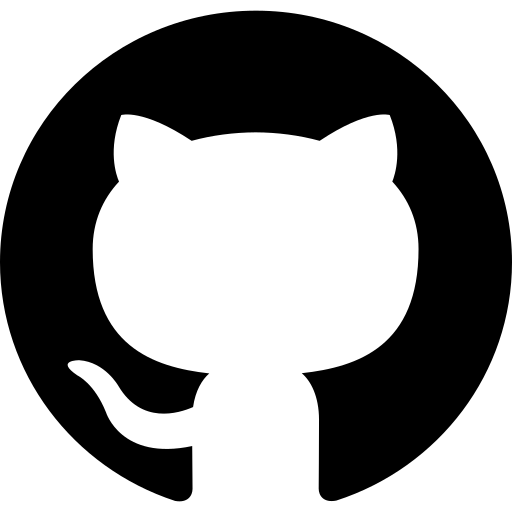
\includegraphics[width=.8\linewidth]{Figure_1}
\caption{Placeholder image with a long example caption to show justification setting.}
\label{fig:computerNo}
\end{figure}

\Blindtext

Figure \ref{fig:computerNo} shows an example of how to insert a column-wide figure. To insert a figure wider than one column, please use the \verb|\begin{figure*}...\end{figure*}| environment. Figures wider than one column should be sized to 11.4 cm or 17.8 cm wide. Use \verb|\begin{SCfigure*}...\end{SCfigure*}| for a wide figure with side captions.

\vspace{1em}
\begin{table}[htp]
\begin{center}
\caption[Example results table]{Example results table, following the same layout used across my thesis chapters. Placeholder values.}
\label{tab:example}
\begin{tabular}{clclc}
\hline
Method &  & Metric &  & Value \\ \hline
\multicolumn{1}{l}{} & & \multicolumn{1}{l}{} & & \multicolumn{1}{l}{} \\

Baseline & & Accuracy & & 87.2\% \\

\multicolumn{1}{l}{} & & \multicolumn{1}{l}{} & & \multicolumn{1}{l}{} \\

Proposed & & Accuracy & & 94.6\% \\

\multicolumn{1}{l}{} & & \multicolumn{1}{l}{} & & \multicolumn{1}{l}{} \\

Proposed & & Latency (ms) & & 12.4 \\

\hline
\end{tabular}
\end{center}
\end{table}

Table \ref{tab:example} shows an example of how to insert a results table using the same style as the thesis: a centered \texttt{tabular} with horizontal rules and blank spacer rows between entries.

\input{sections/discussion}
\section*{Conclusions}

blablaba \ref{fig:computerNo}
\blindtext

\subsection*{Future Work}
\blindtext


\section*{Bibliography}
\bibliography{bib/references}

%% You can use these special %TC: tags to ignore certain parts of the text.
%TC:ignore
%the command above ignores this section for word count
\onecolumn
\newpage

%%%%%%%%%%%%%%%%%%%%%%%%%%%%%
% Supplementary Information %
%%%%%%%%%%%%%%%%%%%%%%%%%%%%%
\captionsetup*{format=largeformat}
\section{Something about something} \label{note:Note1}
\Blindtext


%TC:endignore
%the command above ignores this section for word count

\end{document}
